\section*{Appendix} 

\subsection{Neural Neural Textures: More Details}

	In section \ref{sec:neural_tex}, we mentioned that neural neural textures learn better than raster neural textures. 
	TRITON can be ablated to use raster textures. Let's call this version ``Raster TRITON''. 
	Raster TRITON is extremely sensitive to the resolution of its neural texture, and can be numerically unstable if that resolution is too high.
	In comparison, regular TRITON's neural neural textures don't have a specific resolution: they are continuously defined over the UV domain using fourier feature networks.

	\begin{figure}[H]
		\begin{center}
			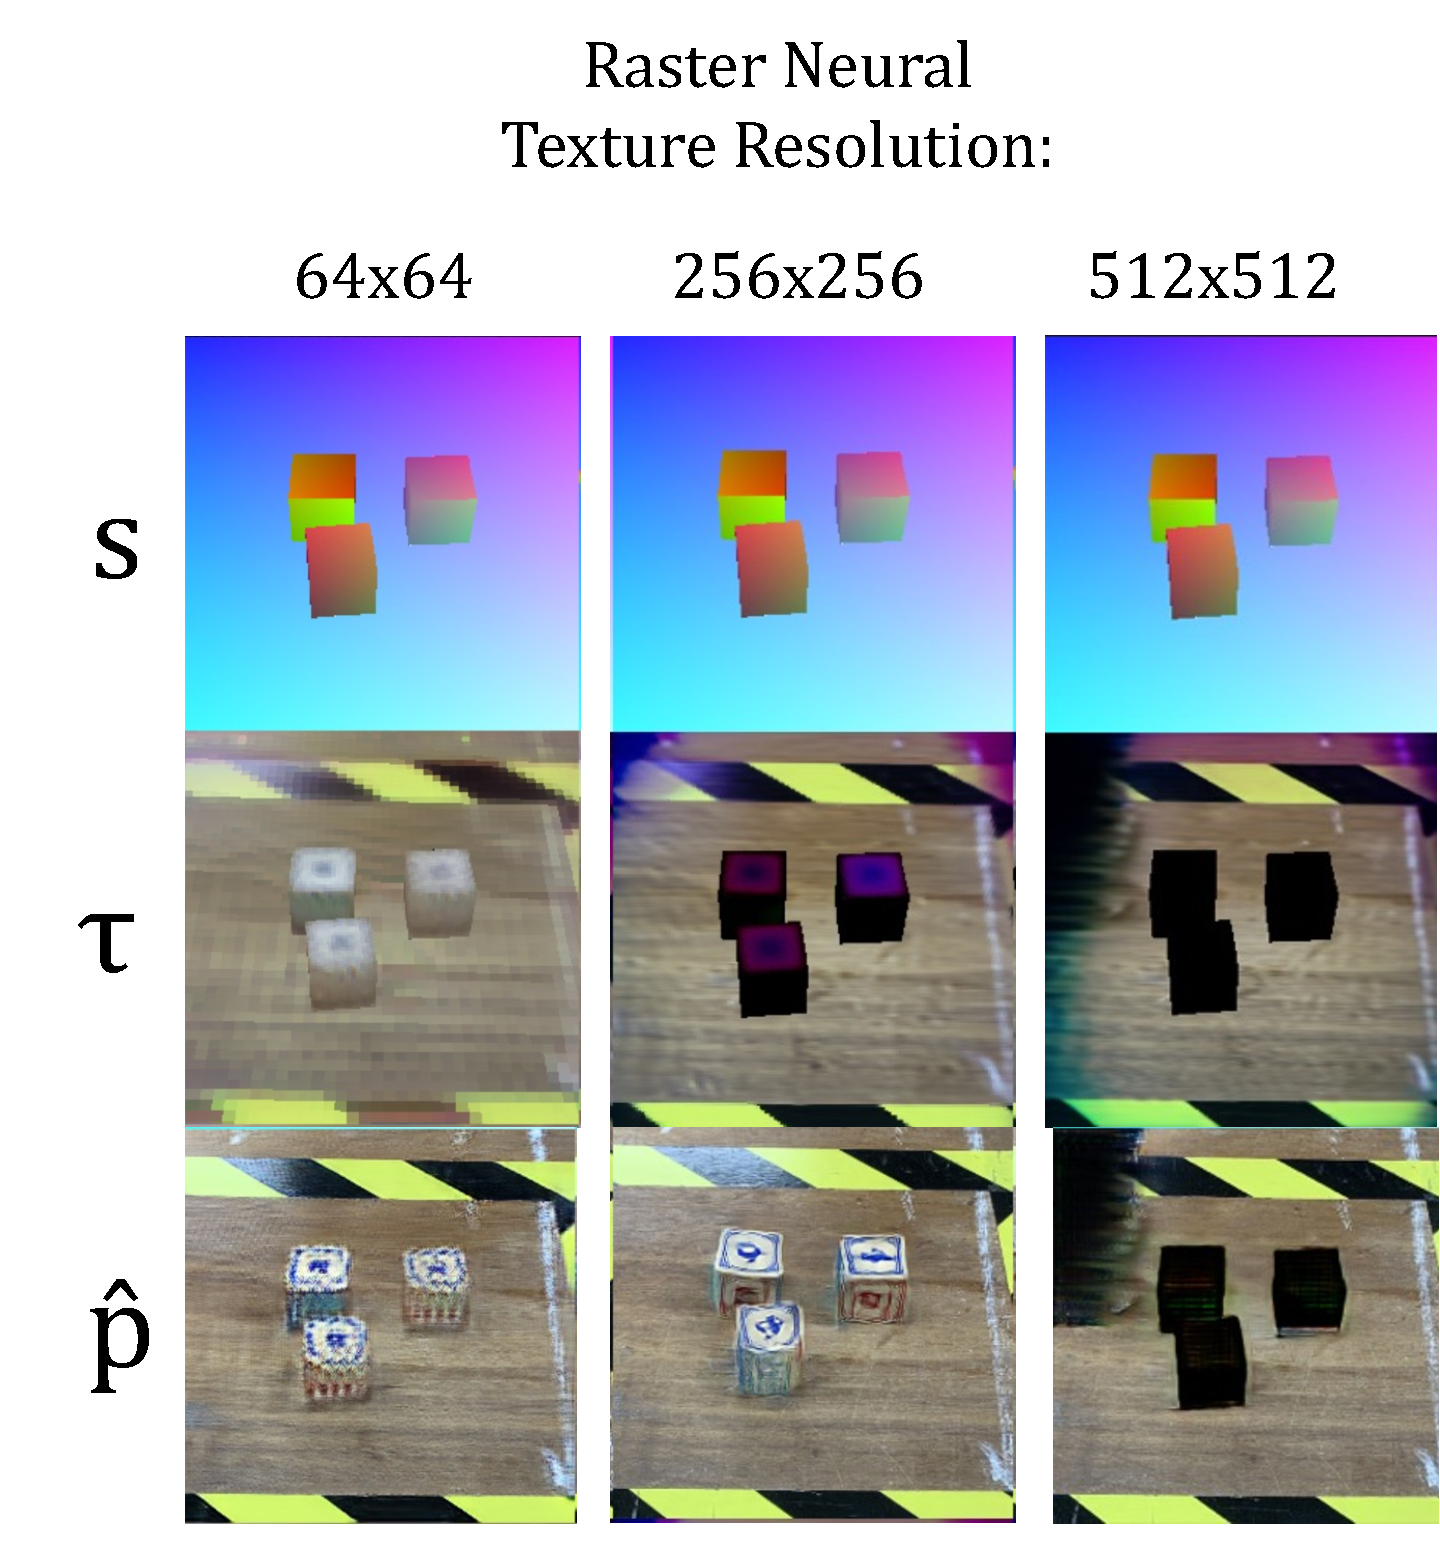
\includegraphics[width=230pt]{../images/raster_texture_resolution_comparisons.pdf}
		\end{center}
		\caption{
			The resolution of the raster neural texture seriously impacts performance in ``Raster TRITON''. Each column has a different neural texture resolution.
			The neural texture only looks like the translation when the resolution is low.
		}
		\label{fig:raster_texture_resolution_comparisons}
	\end{figure}

	In this paragraph we offer possible explanations for these observations.
	With raster-based textures, only the side of an object that currently is seen in a view is allowed to change during each update, because the gradient can't be propogated into pixels that aren't seen.
	If this means changing overall brightness of an object for example, the brightness of that object can't be changed over the entire object until every side has been seen - which won't happen in a single iteration, since the batch size is limited.

	In addition to not propogating the gradient to unseen sides of objects, it also can't propogate to texels in-between the UVL values seen in a scene image.
	When the raster neural texture is too large, aliasing effects occur: if you have a raster texture with very high resolution, the loss gradient is less likely to be passed to a given texel because the chance that a given UV value in a scene will be rounded to that pixel's coordinates is very small.
	In practice, this makes large raster neural textures unstable and limits us to using small amounts of detail.
	With neural neural textures, this aliasing problem is mostly mitigated, because when a certain texture receives a gradient at particular UV coordinates, the areas of the texture between those coordinates are also changed.

\subsection{Unprojection Consistency Loss: More Details}

	Here, we give more details about unprojection consistency loss $\lUC$.

	The exact equation for $\lUC$ is as follows:
	to formally define $\lUC$ we define unprojections $\unprojection^{1...N,1...L}$ and mean unprojections (aka recovered textures) $\bar{\unprojection}^{1...L}$ 
	with each $\unprojection^{n,i}\in\real^{3\times128\times128}$:
	%Jinghyan's Version (uses expectation)
	% \begin{equation}
	% 	\unprojection_{U,V}^{n,i}=\expectation\ph_{x,y}^n 
	% 	\eqand \bar{\unprojection}^i_{u,v}   =   
	% 		\frac{1}{N} \lsum_n\unprojection^{n,i}_{u,v} 
	% 	\eqand 
	% 	%\lUC=\frac{\lsum_{i,U,V}
	% 	%\sqrt[]{\frac{1}{N}\lsum_n\left(\bar{\unprojection}^i_{u,v}-\unprojection^{i,n}_{U,V}\right)^2}}
	% 	%{128\cdot128\cdot L}
	% 	\lUC=\mathbb{E}\left[
	% 	\sqrt[]{\frac{1}{N}\lsum_n\left(\bar{\unprojection}^i_{u,v}-\unprojection^{i,n}_{U,V}\right)^2} \right]
	% \end{equation}
	%
	%
	%Unabbreviated: Not Jinguan's version; 
% 	\resizebox{\textwidth}{!}{
	\begin{equation}
		\unprojection_{c,U,V}^{n,i}=\expectation\ph_{c,x,y}^n 
		\eqand \bar{\unprojection}^i_{c,u,v}   =   
			\frac{1}{N} \lsum_{n=1}^N\unprojection^{n,i}_{c,u,v} 
		\eqand 
		\lUC=\frac{\lsum_{i=1}^L\lsum_{c=1}^3\lsum_{U=1}^{128}\lsum_{V=1}^{128}
		\sqrt[]{\frac{1}{N}\lsum_{n=1}^N\left(\bar{\unprojection}^i_{c,u,v}-\unprojection^{i,n}_{c,U,V}\right)^2}}
		{3\cdot128\cdot128\cdot L}
	\end{equation}
% 	}
	where $U=\lfloor128u\rfloor$ and $V=\lfloor128v\rfloor$ and $i=I(l)$ with
	%  $(u,v,l)=s^n_{1...3,x,y}$
	$u=s^n_{1,x,y}$, $v=s^n_{2,x,y}$, $l=s^n_{3,x,y}$
	for all 
	$n \in \{1...N\}$ , 
	$i \in \{1...L\}$ , 
	$x \in \{1...W\}$ , 
	$y \in \{1...H\}$ , 
	$U \in \{1...128\}$ , 
	$V \in \{1...128\}$.

	\bigskip
	
	The hyperparameter 128 we described in section \ref{sec:unprojection_consistency_loss} refers to the resolution of the unprojections used to calculate $\lUC$.
	In figure \ref{fig:unprojection_resolution_comparison} we see that if we were to set it higher, the gradient wouldn't affect the neural texture as densely.

	\begin{figure}[H]
		\begin{center}
			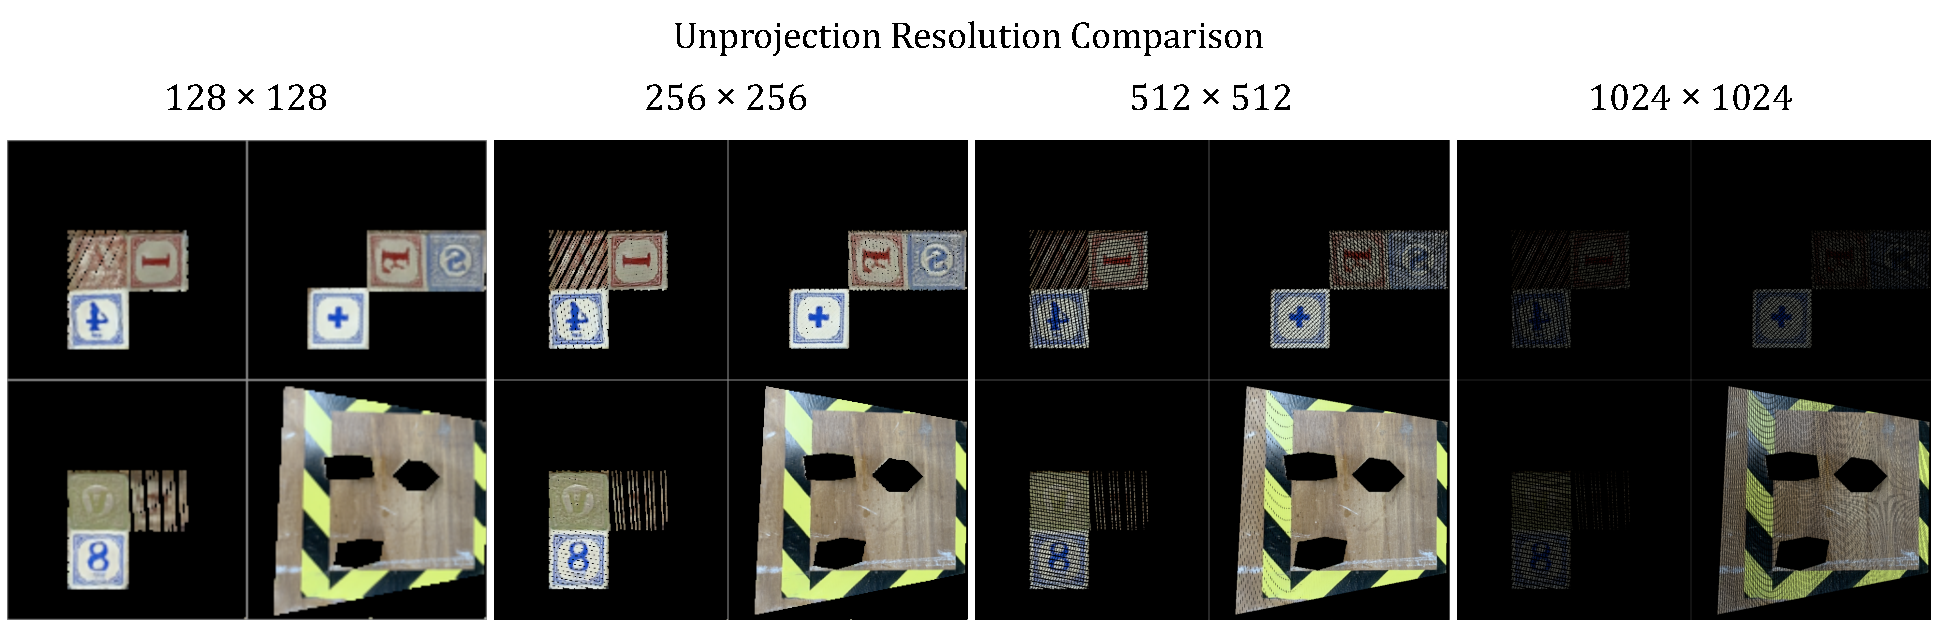
\includegraphics[width=400pt]{../images/unprojection_resolution_comparison.pdf}
		\end{center}
		\caption{
			Here, we unproject a single translation $\ph^i$. The resolution of the unprojection matters for unprojection consistency loss. The larger it is, the more precise the alignment will be but the less likely a given UV value is to be assigned a loss greater than 0, creating numerical instability and slowing down learning. 
			When the unprojection resolution is too high, only a few areas of the neural texture will receive a gradient during backpropogation. In practice we use the resolution $128\times128$.
		}
		\label{fig:unprojection_resolution_comparison}
	\end{figure}

\subsection{More Results}